\documentclass[ExampleMasters.tex]{subfiles}
%\documentclass{article}
%\usepackage{amsmath}
%\usepackage{graphicx}
%\usepackage[margin=1.3in]{geometry}
%\usepackage{float}
%\usepackage{caption}
%\usepackage{subcaption}
\begin{document}
%\centerline{\sc \large Long combinations with additional electric propulsion}
%\vspace{.5pc}
%\centerline{\sc Model validation results}
%\centerline{Karthik Venkataraman, 880128-T539}
%\listoffigures
\chapter{Optimisation Results}

\section{Introduction}
As set out in the abstract, the generic vehicle model described in the Chapter 4 is used in consonance with the genetic algorithm described in Chapter 2 to derive optimal vehicle propulsion configurations for years 2015, 2020, 2025 and 2030, the objective function optimised being the vehicle productivity over the lifetime of the first owner's holding.\\

In this chapter, the results of the optimisation shall be presented in four different sub-sections. The first contains a brief listing of the results derived from successive runs of the genetic algorithm lasting 100 generations each. The following subsections are an analysis of the results in different headings.

\section{Overview of the results}
Optimal axle propulsion configurations are derived for the years specified above. The following tables list the results for varying gross combination weights of 50t, 60t, 70t and 80t for each of the four years in succession.

\begin{table}[ht]
\caption{Optimal combination configurations - Year 2015}
\centering
\begin{tabular}{c c c c c c}
\hline\hline
GCW & \multicolumn{4}{c}{Optimal configuration} & Vehicle Productivity \\ \cline{2-5}
(t) & Tractor & Semi-trailer & Dolly & Semi-trailer & (\euro/\euro)\\ 
\hline
50 & 010\textbackslash000\textbackslash011 &
	 001\textbackslash001\textbackslash000 & 100\textbackslash001\textbackslash00 &
	 100\textbackslash001\textbackslash000 & 0.960028 \\
60 & 100\textbackslash000\textbackslash011 &
	 001\textbackslash100\textbackslash001 & 010\textbackslash010\textbackslash00 &
	 010\textbackslash100\textbackslash000 & 1.25954 \\
70 & 100\textbackslash000\textbackslash011 & 
	 001\textbackslash100\textbackslash110 & 010\textbackslash001\textbackslash00  & 
	 100\textbackslash010\textbackslash000 & 1.49906 \\
80 & 100\textbackslash000\textbackslash011 &
	 100\textbackslash010\textbackslash000 & 100\textbackslash100\textbackslash00 &
	 001\textbackslash100\textbackslash011 & 1.80818 \\
\hline
\end{tabular}
\label{table:optComb2015}
\end{table}

\begin{table}[ht]
\caption{Optimal combination configurations - Year 2020}
\centering
\begin{tabular}{c c c c c c}
\hline\hline
GCW & \multicolumn{4}{c}{Optimal configuration} & Vehicle Productivity \\ \cline{2-5}
(t) & Tractor & Semi-trailer & Dolly & Semi-trailer & (\euro/\euro)\\ 
\hline
50 & 100\textbackslash000\textbackslash011 &
	 100\textbackslash100\textbackslash000  & 001\textbackslash001\textbackslash00  & 
	 001\textbackslash100\textbackslash010 & 0.974871 \\
60 & 100\textbackslash000\textbackslash011 & 
	 001\textbackslash100\textbackslash001 & 100\textbackslash010\textbackslash00 &
	 100\textbackslash010\textbackslash000 & 1.27334 \\
70 & 100\textbackslash000\textbackslash011 &
	 001\textbackslash100\textbackslash101 & 100\textbackslash100\textbackslash00 &
	 001\textbackslash010\textbackslash000 & 1.49906 \\
80 & 100\textbackslash000\textbackslash011 & 
	 001\textbackslash100\textbackslash011 & 010\textbackslash100\textbackslash00 &
	 001\textbackslash001\textbackslash000 & 1.80818 \\
\hline
\end{tabular}
\label{table:optComb2020}
\end{table}

\begin{table}[ht]
\caption{Optimal combination configurations - Year 2025}
\centering
\begin{tabular}{c c c c c c}
\hline\hline
GCW & \multicolumn{4}{c}{Optimal configuration} & Vehicle Productivity \\ \cline{2-5}
(t) & Tractor & Semi-trailer & Dolly & Semi-trailer & (\euro/\euro)\\ 
\hline
50 & 100\textbackslash000\textbackslash011 & 001\textbackslash100\textbackslash100 & 100\textbackslash010\textbackslash00 & 100\textbackslash100\textbackslash000 & 0.984204 \\
60 & 100\textbackslash000\textbackslash011 & 001\textbackslash100\textbackslash011 & 100\textbackslash100\textbackslash00 & 100\textbackslash001\textbackslash000 & 1.28676 \\
70 & 100\textbackslash000\textbackslash011 & 001\textbackslash100\textbackslash000 & 100\textbackslash100\textbackslash00 & 001\textbackslash100\textbackslash011 & 1.5351 \\
80 & 100\textbackslash000\textbackslash011 & 001\textbackslash100\textbackslash111 & 001\textbackslash010\textbackslash00 & 010\textbackslash100\textbackslash000 & 1.8501 \\
\hline
\end{tabular}
\label{table:optComb2025}
\end{table}

\begin{table}[ht]
\caption{Optimal combination configurations - Year 2030}
\centering
\begin{tabular}{c c c c c c}
\hline\hline
GCW & \multicolumn{4}{c}{Optimal configuration} & Vehicle Productivity \\ \cline{2-5}
(t) & Tractor & Semi-trailer & Dolly & Semi-trailer & (\euro/\euro)\\ 
\hline
50 & 100\textbackslash000\textbackslash011 & 100\textbackslash100\textbackslash000 & 001\textbackslash100\textbackslash01 & 001\textbackslash010\textbackslash000 & 0.99445 \\
60 & 100\textbackslash000\textbackslash011 & 001\textbackslash100\textbackslash000 & 010\textbackslash100\textbackslash00 & 001\textbackslash100\textbackslash011 & 1.30212 \\
70 & 100\textbackslash000\textbackslash011 & 001\textbackslash100\textbackslash010 & 001\textbackslash010\textbackslash00 & 001\textbackslash100\textbackslash010 & 1.55402 \\
80 & 100\textbackslash000\textbackslash011 & 001\textbackslash010\textbackslash000 & 001\textbackslash100\textbackslash01 & 001\textbackslash100\textbackslash101 & 1.87496 \\
\hline
\end{tabular}
\label{table:optComb2030}
\end{table}

As can be seen, the engine tends to be downsized from the D16 to the D13 and D11 variants complemented by increased axle electrification. An detailed analysis of the results follows.\\

\section{Comparison with conventional combinations}
Combinations that are powered only by the engine are chosen as a 'base' variant and compared with the optimal configuration for each GCW across the years. As can be seen, the fuel savings resulting from axle electrification and comapritively smaller driver wages owing to shorter mission times consistently drive the productivity higher. For example, the optimal configuration for the 50t combination in the year 2015 is compared with the standard A-Double driven by the D16 engine variant. The fixed and variable costs are compared between the two combinations to motivate the increased mission productivity. As can be seen in Figure \ref{2015A0vsA1}, reduced fuel consumption in case of the D13 variant as well as reduced powertrain prices can be related to improved productivity.\\

\begin{figure}
\centering
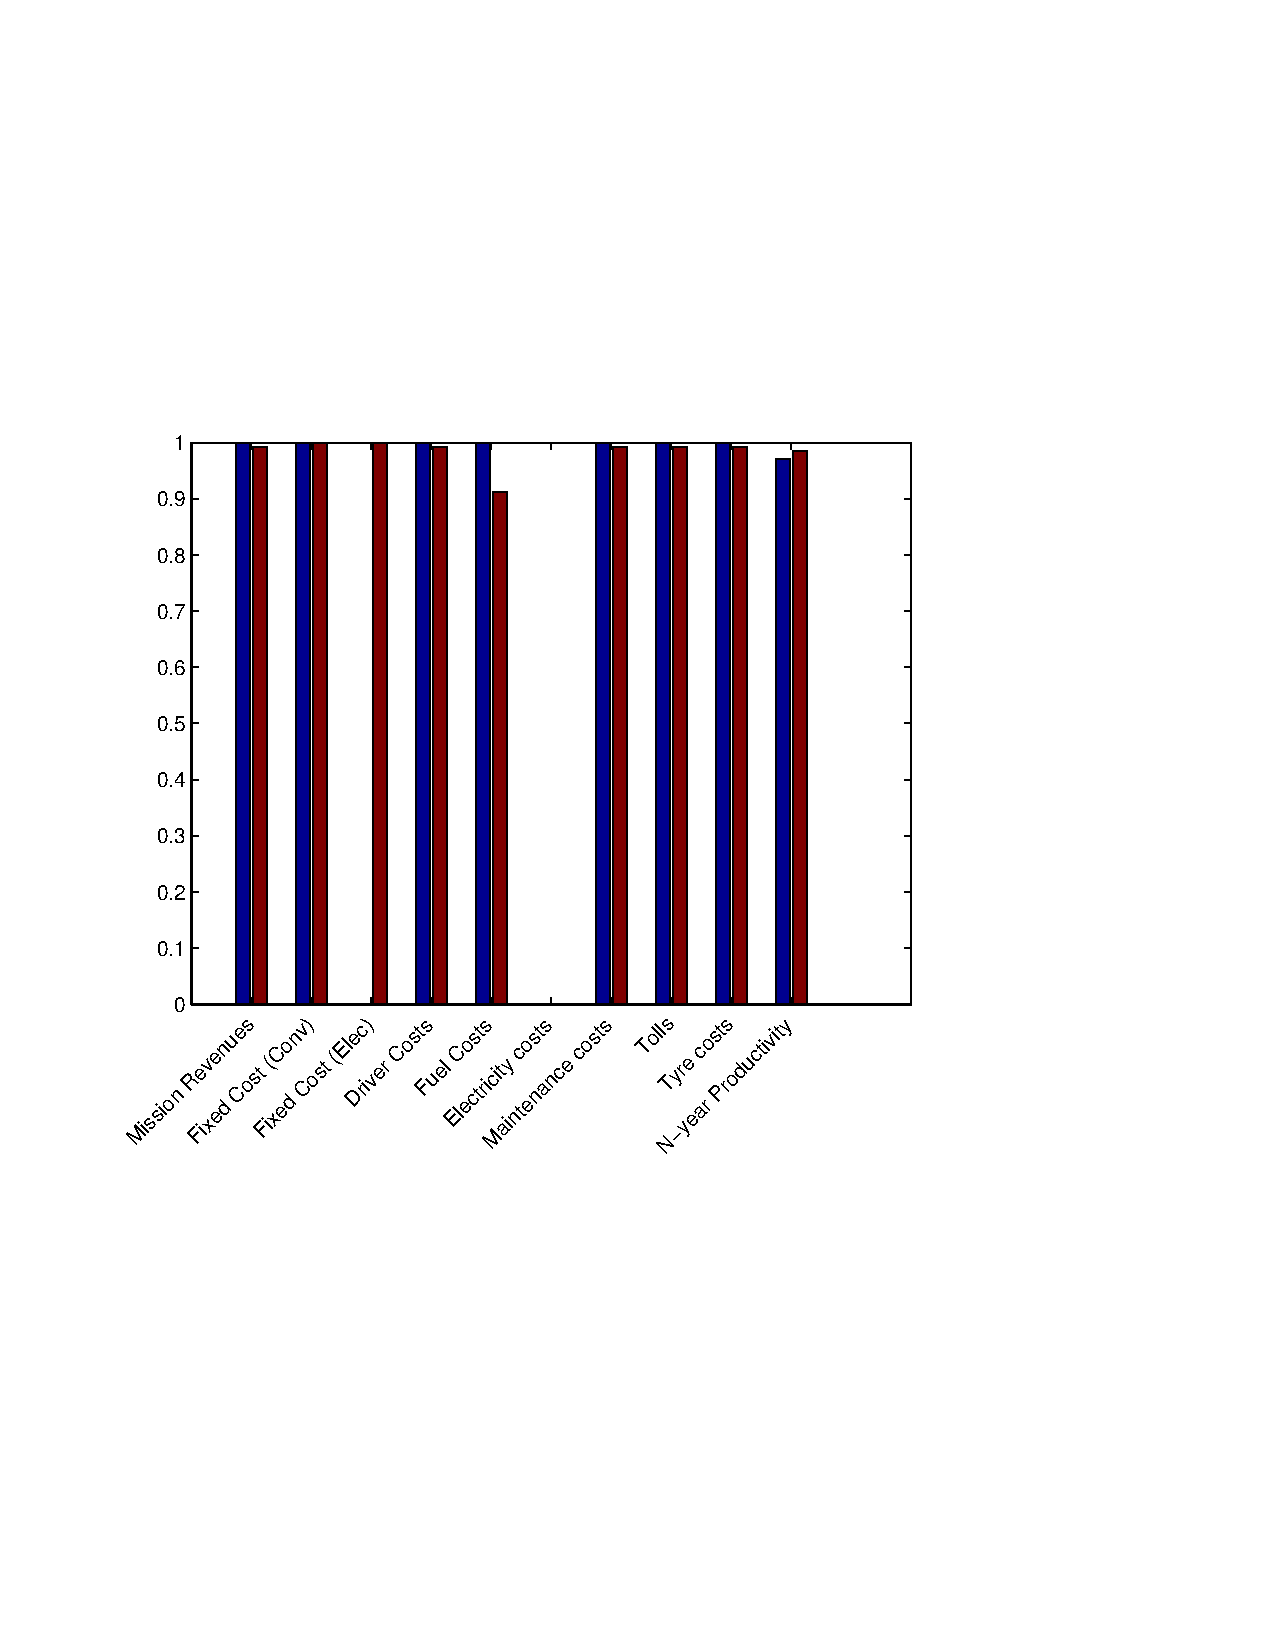
\includegraphics[width=0.7\textwidth, clip=true, trim=45 225 125 208]{figures/OptimalCombinationResults/2015/A.pdf}
\caption{D13 powered A-Double (Optimal) vs standard D16 powered A-Double (Base)}
\label{2015A0vsA1}
\end{figure}

The fuel savings and driver wage advantages are more visible for higher GCWs such as the one shown in Figure \ref{2015C0vsC1} for a GCW of 70t.\\

\begin{figure}
\centering
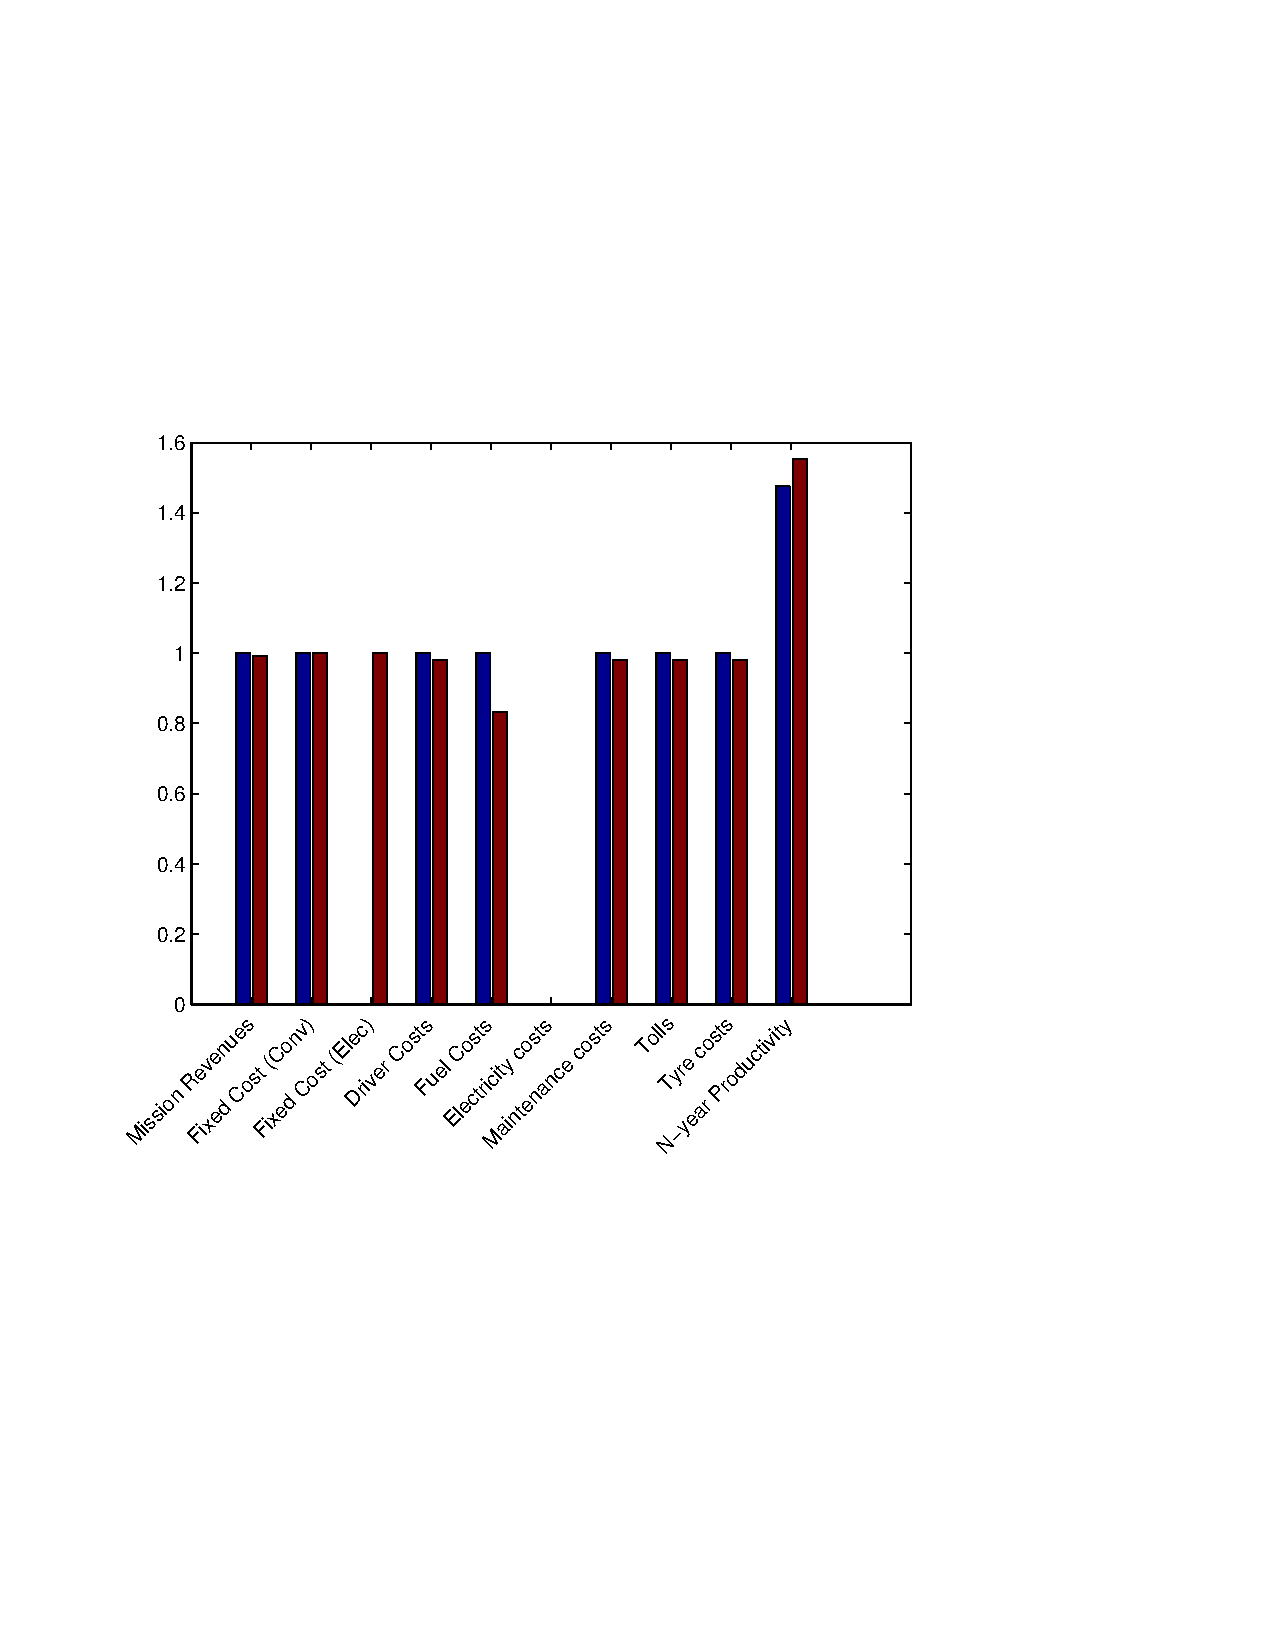
\includegraphics[width=0.7\textwidth, clip=true, trim=45 225 125 208]{figures/OptimalCombinationResults/2015/C.pdf}
\caption{Optimal 70t combination vs D11 powered A-Double (Base)}
\label{2015C0vsC1}
\end{figure}

\end{document}